% Options for packages loaded elsewhere
% Options for packages loaded elsewhere
\PassOptionsToPackage{unicode}{hyperref}
\PassOptionsToPackage{hyphens}{url}
\PassOptionsToPackage{dvipsnames,svgnames,x11names}{xcolor}
%
\documentclass[
  11pt,
]{article}
\usepackage{xcolor}
\usepackage[margin=1in]{geometry}
\usepackage{amsmath,amssymb}
\setcounter{secnumdepth}{5}
\usepackage{iftex}
\ifPDFTeX
  \usepackage[T1]{fontenc}
  \usepackage[utf8]{inputenc}
  \usepackage{textcomp} % provide euro and other symbols
\else % if luatex or xetex
  \usepackage{unicode-math} % this also loads fontspec
  \defaultfontfeatures{Scale=MatchLowercase}
  \defaultfontfeatures[\rmfamily]{Ligatures=TeX,Scale=1}
\fi
\usepackage{lmodern}
\ifPDFTeX\else
  % xetex/luatex font selection
\fi
% Use upquote if available, for straight quotes in verbatim environments
\IfFileExists{upquote.sty}{\usepackage{upquote}}{}
\IfFileExists{microtype.sty}{% use microtype if available
  \usepackage[]{microtype}
  \UseMicrotypeSet[protrusion]{basicmath} % disable protrusion for tt fonts
}{}
\usepackage{setspace}
\makeatletter
\@ifundefined{KOMAClassName}{% if non-KOMA class
  \IfFileExists{parskip.sty}{%
    \usepackage{parskip}
  }{% else
    \setlength{\parindent}{0pt}
    \setlength{\parskip}{6pt plus 2pt minus 1pt}}
}{% if KOMA class
  \KOMAoptions{parskip=half}}
\makeatother
% Make \paragraph and \subparagraph free-standing
\makeatletter
\ifx\paragraph\undefined\else
  \let\oldparagraph\paragraph
  \renewcommand{\paragraph}{
    \@ifstar
      \xxxParagraphStar
      \xxxParagraphNoStar
  }
  \newcommand{\xxxParagraphStar}[1]{\oldparagraph*{#1}\mbox{}}
  \newcommand{\xxxParagraphNoStar}[1]{\oldparagraph{#1}\mbox{}}
\fi
\ifx\subparagraph\undefined\else
  \let\oldsubparagraph\subparagraph
  \renewcommand{\subparagraph}{
    \@ifstar
      \xxxSubParagraphStar
      \xxxSubParagraphNoStar
  }
  \newcommand{\xxxSubParagraphStar}[1]{\oldsubparagraph*{#1}\mbox{}}
  \newcommand{\xxxSubParagraphNoStar}[1]{\oldsubparagraph{#1}\mbox{}}
\fi
\makeatother


\usepackage{longtable,booktabs,array}
\usepackage{calc} % for calculating minipage widths
% Correct order of tables after \paragraph or \subparagraph
\usepackage{etoolbox}
\makeatletter
\patchcmd\longtable{\par}{\if@noskipsec\mbox{}\fi\par}{}{}
\makeatother
% Allow footnotes in longtable head/foot
\IfFileExists{footnotehyper.sty}{\usepackage{footnotehyper}}{\usepackage{footnote}}
\makesavenoteenv{longtable}
\usepackage{graphicx}
\makeatletter
\newsavebox\pandoc@box
\newcommand*\pandocbounded[1]{% scales image to fit in text height/width
  \sbox\pandoc@box{#1}%
  \Gscale@div\@tempa{\textheight}{\dimexpr\ht\pandoc@box+\dp\pandoc@box\relax}%
  \Gscale@div\@tempb{\linewidth}{\wd\pandoc@box}%
  \ifdim\@tempb\p@<\@tempa\p@\let\@tempa\@tempb\fi% select the smaller of both
  \ifdim\@tempa\p@<\p@\scalebox{\@tempa}{\usebox\pandoc@box}%
  \else\usebox{\pandoc@box}%
  \fi%
}
% Set default figure placement to htbp
\def\fps@figure{htbp}
\makeatother





\setlength{\emergencystretch}{3em} % prevent overfull lines

\providecommand{\tightlist}{%
  \setlength{\itemsep}{0pt}\setlength{\parskip}{0pt}}



 
\usepackage[]{biblatex}
\addbibresource{references.bib}


\usepackage{hyperref}
\hypersetup{
  colorlinks=true,
  linkcolor=blue,
  urlcolor=blue,
  breaklinks=true,
  pdfborder={0 0 0}
}
\makeatletter
\@ifpackageloaded{caption}{}{\usepackage{caption}}
\AtBeginDocument{%
\ifdefined\contentsname
  \renewcommand*\contentsname{Table of contents}
\else
  \newcommand\contentsname{Table of contents}
\fi
\ifdefined\listfigurename
  \renewcommand*\listfigurename{List of Figures}
\else
  \newcommand\listfigurename{List of Figures}
\fi
\ifdefined\listtablename
  \renewcommand*\listtablename{List of Tables}
\else
  \newcommand\listtablename{List of Tables}
\fi
\ifdefined\figurename
  \renewcommand*\figurename{Figure}
\else
  \newcommand\figurename{Figure}
\fi
\ifdefined\tablename
  \renewcommand*\tablename{Table}
\else
  \newcommand\tablename{Table}
\fi
}
\@ifpackageloaded{float}{}{\usepackage{float}}
\floatstyle{ruled}
\@ifundefined{c@chapter}{\newfloat{codelisting}{h}{lop}}{\newfloat{codelisting}{h}{lop}[chapter]}
\floatname{codelisting}{Listing}
\newcommand*\listoflistings{\listof{codelisting}{List of Listings}}
\makeatother
\makeatletter
\makeatother
\makeatletter
\@ifpackageloaded{caption}{}{\usepackage{caption}}
\@ifpackageloaded{subcaption}{}{\usepackage{subcaption}}
\makeatother
\usepackage{bookmark}
\IfFileExists{xurl.sty}{\usepackage{xurl}}{} % add URL line breaks if available
\urlstyle{same}
\hypersetup{
  pdftitle={William's Update},
  pdfauthor={William Clinton Co},
  colorlinks=true,
  linkcolor={blue},
  filecolor={Maroon},
  citecolor={blue},
  urlcolor={blue},
  pdfcreator={LaTeX via pandoc}}


\title{William's Update}
\usepackage{etoolbox}
\makeatletter
\providecommand{\subtitle}[1]{% add subtitle to \maketitle
  \apptocmd{\@title}{\par {\large #1 \par}}{}{}
}
\makeatother
\subtitle{Remittances}
\author{William Clinton Co}
\date{August 11, 2025}
\begin{document}
\maketitle
\begin{abstract}
This paper examines the current environment of remittance measurement,
identifying key literature and data sources while also addressing topics
discussed during William and Michael's meeting on July 24, 2025.
\end{abstract}

\renewcommand*\contentsname{Table of contents}
{
\hypersetup{linkcolor=}
\setcounter{tocdepth}{3}
\tableofcontents
}

\setstretch{1}
\section{Introduction}\label{introduction}

In general the remitance datasets are weak. I will be presenting the
followign options which would be the best avaialbel datasets out there
on remitances.

\section{Email Communications}\label{email-communications}

I contacted Remitly and Wise for data access requests.

\section{Best Dataset is World Bank}\label{best-dataset-is-world-bank}

\subsection{Cost of Remittances
Dataset}\label{cost-of-remittances-dataset}

This is a more comprehensive dataset. Please see the
\href{https://github.com/WilliamClintC/RER/blob/main/data/Remittance_2/rpw_dataset_2011_2024_q3.xlsx}{sample
dataset} where we can observe source and destination countries.

We can also observe the firm, payment instrument (bank transfer, cash,
etc.), and speed.

There are many different methodologies with regards to remittances. For
an overview, please see the
\href{https://remittanceprices.worldbank.org/resources}{World Bank's
resources page}.

The best dataset would be from the World Bank, as they seek to establish
a unified standard for remittances and maintain public data
availability. See
\href{https://remittanceprices.worldbank.org/national-and-regional-databases-certified-by-the-world-bank}{national
and regional databases certified by the World Bank}.

There is a problem with their data request site maybe you can try as
well. I have sent them several requests with no instructions being
received. The dataset should be available at:
\href{https://remittanceprices.worldbank.org/file-download/remittance-prices-worldwide-2011-2024q3-dataset}{World
Bank Remittance Prices Dataset}

\subsection{Remittances Sent Dataset}\label{remittances-sent-dataset}

We have the following fields available in the screenshot below:

\begin{figure}[H]

{\centering \pandocbounded{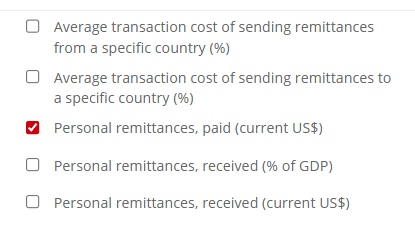
\includegraphics[keepaspectratio]{images/Screenshot 2025-08-07 063601.png}}

}

\caption{Available Fields for Remittances Sent Dataset}

\end{figure}%

We are not able to observe bilateral remittance flows; we can only
observe aggregates unlike the cost dataset. Bilateral flows are like
this - I can't seem to find the bilateral dataset anymore. I think they
stopped sharing it. The dataset is available in the reports, but that's
about it.

According to the literature: ``Additionally, the World Bank also
publishes estimates on bilateral remittance flows. The basis for
bilateral remittances estimates are weighted migrant stock data, the
weighted income of migrants based on the per capita income in the
country of destination, and the weighted income in the origin country of
the migrant (Ratha and Shaw, 2007: 43).''

The main dataset can be found at:
\href{https://databank.worldbank.org/metadataglossary/world-development-indicators/series/BM.TRF.PWKR.CD.DT}{World
Bank Development Indicators - Personal Remittances}

It is not perfect - see the limitations at the
\href{https://databank.worldbank.org/metadataglossary/world-development-indicators/series/BM.TRF.PWKR.CD.DT}{World
Bank metadata page}, but it's the best we have.

\begin{quote}
Because direct measurement (tracking actual transactions) is often
incomplete, they use a mix of methods: Direct reporting when possible
and estimates and models to fill in gaps.
\end{quote}

\subsection{Remitscope}\label{remitscope}

It may be worthwhile to consider
\href{https://remitscope.org/latin-america/themes/}{RemitScope} as an
additional resource. PLease see this to see hwo to use remitscope
https://remitscope.org/how-to-use-remitscope/

RemitScope I think is our best bet given that they aggregate all
different sources of remittances. From my understanding the remittances
bilateral data exist but they do not exist in an easily accessible
format. RemitScope aggregates the data into a format that's accessible.

This is a quote from the website:

\begin{quote}
RemitSCOPE brings together data from secondary sources, that are usually
scattered in different organisations and agencies, as well as collecting
data through primary research and directly from market operators and
regulators.
\end{quote}

The dataset currently covers Africa and Latin America. Asia is coming
soon - please see this image:

\begin{figure}[H]

{\centering \pandocbounded{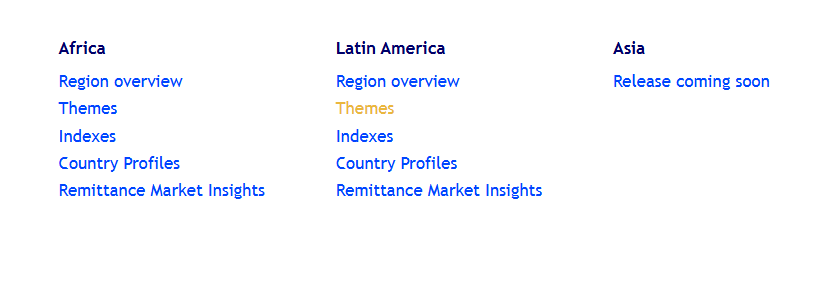
\includegraphics[keepaspectratio]{images/Screenshot 2025-08-11 005134.png}}

}

\caption{RemitScope Regional Coverage}

\end{figure}%

Please see this useful dataset. It is very detailed and shows us what
datasets are available out there, to what detail, and from what source:

\href{https://remitscope.org/wp-content/uploads/2023/08/RemitSCOPE-Thematic-Dashboards-Overview.pdf}{RemitSCOPE
Thematic Dashboards Overview}

Please see this image:

\begin{figure}[H]

{\centering \pandocbounded{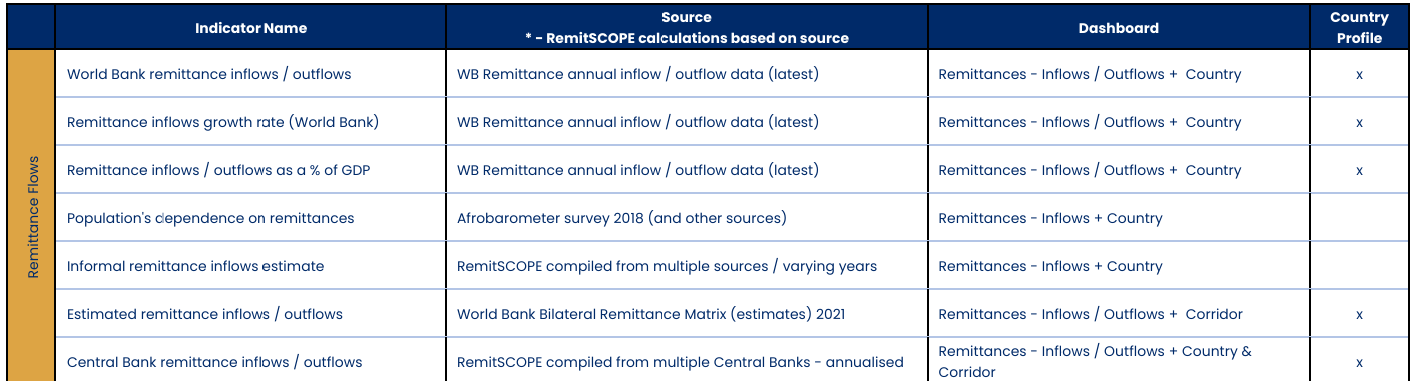
\includegraphics[keepaspectratio]{images/Screenshot 2025-08-11 010105.png}}

}

\caption{RemitSCOPE Dataset Overview}

\end{figure}%

Currently RemitScope only allows for observation through visualizations.
I can scrape data from this website if need be.

See this image of an example visualization from RemitScope:

\begin{figure}[H]

{\centering \pandocbounded{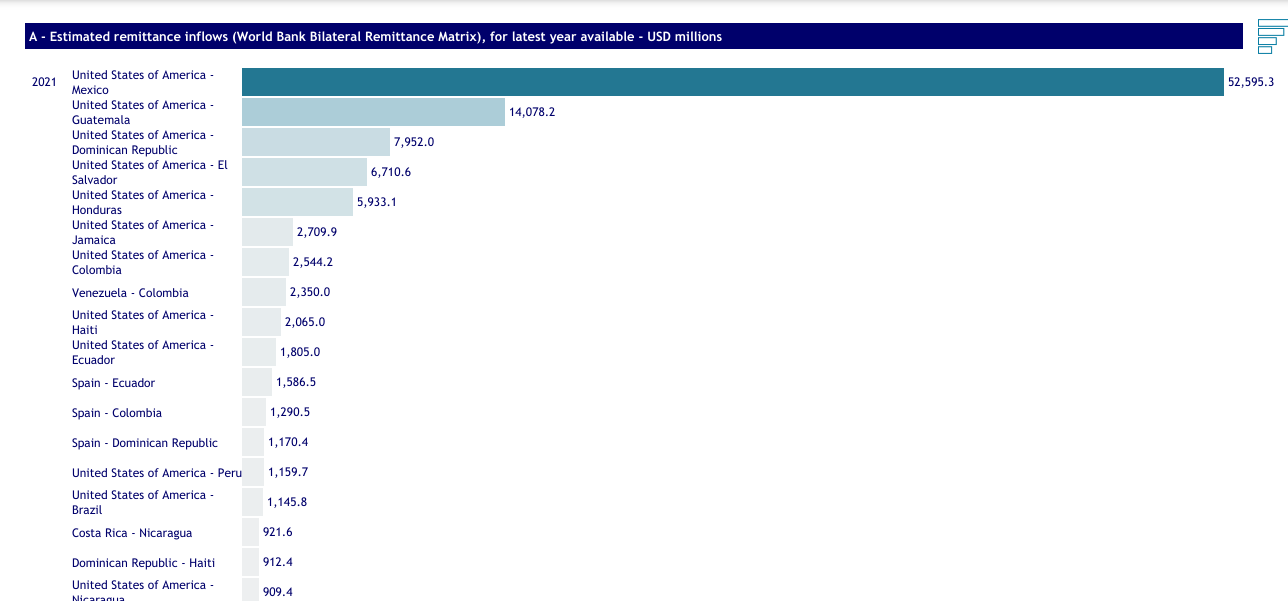
\includegraphics[keepaspectratio]{images/Screenshot 2025-08-11 014421.png}}

}

\caption{RemitScope Example Visualization}

\end{figure}%

See this link to go to the website and see for oneself:
\href{https://remitscope.org/latin-america/themes/}{RemitScope Latin
America Themes}

\subsection{Canadian International Development Platform:
CIDP}\label{canadian-international-development-platform-cidp}

The \href{https://cidpnsi.ca/remittances-explorer/}{CIDP Remittances
Explorer} is a Canadian International Development Platform tool that
uses World Bank datasets as a derivative source to create an interactive
remittance data visualization website.

\subsection{Additional Data Sources}\label{additional-data-sources}

\begin{itemize}
\tightlist
\item
  \href{https://sdgstoday.org/dataset/remittances}{SDGs Today
  Remittances Dataset} - Sustainable Development Goals tracking platform
  for remittance data
\end{itemize}

\subsection{Data Request Status}\label{data-request-status}

I have submitted a data request through the
\href{https://remittanceprices.worldbank.org/data-download}{World Bank's
data download portal} to obtain the most current and comprehensive
remittance datasets.

Wise rejected my request - please see the screenshot below:

\begin{figure}[H]

{\centering \pandocbounded{
\includegraphics[keepaspectratio]{images/Screenshot 2025-08-07 153221.png}}

}

\caption{Wise Data Request Rejection}

\end{figure}%


\printbibliography



\end{document}
